\documentclass[hidelinks,12pt]{article}
\usepackage[left=0.25cm,top=1cm,right=0.25cm,bottom=1cm]{geometry}
%\usepackage[landscape]{geometry}
\textwidth = 20cm
\hoffset = -1cm
\usepackage[utf8]{inputenc}
\usepackage[spanish,es-tabla]{babel}
\usepackage[autostyle,spanish=mexican]{csquotes}
\usepackage[tbtags]{amsmath}
\usepackage{nccmath}
\usepackage{amsthm}
\usepackage{amssymb}
\usepackage{mathrsfs}
\usepackage{graphicx}
\usepackage{subfig}
\usepackage{standalone}
\usepackage[outdir=./Imagenes/]{epstopdf}
\usepackage{siunitx}
\usepackage{physics}
\usepackage{color}
\usepackage{float}
\usepackage{hyperref}
\usepackage{multicol}
%\usepackage{milista}
\usepackage{anyfontsize}
\usepackage{anysize}
%\usepackage{enumerate}
\usepackage[shortlabels]{enumitem}
\usepackage{capt-of}
\usepackage{bm}
\usepackage{relsize}
\usepackage{placeins}
\usepackage{empheq}
\usepackage{cancel}
\usepackage{wrapfig}
\usepackage[flushleft]{threeparttable}
\usepackage{makecell}
\usepackage{fancyhdr}
\usepackage{tikz}
\usepackage{bigints}
\usepackage{scalerel}
\usepackage{pgfplots}
\usepackage{pdflscape}
\pgfplotsset{compat=1.16}
\spanishdecimal{.}
\renewcommand{\baselinestretch}{1.5} 
\renewcommand\labelenumii{\theenumi.{\arabic{enumii}})}
\newcommand{\ptilde}[1]{\ensuremath{{#1}^{\prime}}}
\newcommand{\stilde}[1]{\ensuremath{{#1}^{\prime \prime}}}
\newcommand{\ttilde}[1]{\ensuremath{{#1}^{\prime \prime \prime}}}
\newcommand{\ntilde}[2]{\ensuremath{{#1}^{(#2)}}}

\newtheorem{defi}{{\it Definición}}[section]
\newtheorem{teo}{{\it Teorema}}[section]
\newtheorem{ejemplo}{{\it Ejemplo}}[section]
\newtheorem{propiedad}{{\it Propiedad}}[section]
\newtheorem{lema}{{\it Lema}}[section]
\newtheorem{cor}{Corolario}
\newtheorem{ejer}{Ejercicio}[section]

\newlist{milista}{enumerate}{2}
\setlist[milista,1]{label=\arabic*)}
\setlist[milista,2]{label=\arabic{milistai}.\arabic*)}
\newlength{\depthofsumsign}
\setlength{\depthofsumsign}{\depthof{$\sum$}}
\newcommand{\nsum}[1][1.4]{% only for \displaystyle
    \mathop{%
        \raisebox
            {-#1\depthofsumsign+1\depthofsumsign}
            {\scalebox
                {#1}
                {$\displaystyle\sum$}%
            }
    }
}
\def\scaleint#1{\vcenter{\hbox{\scaleto[3ex]{\displaystyle\int}{#1}}}}
\def\bs{\mkern-12mu}


\title{Enunciados del Tema 2 \\[0.3em]  \large{Matemáticas Avanzadas de la Física}\vspace{-3ex}}
\author{M. en C. Gustavo Contreras Mayén}
\date{ }
\begin{document}
\vspace{-4cm}
\maketitle
\fontsize{14}{14}\selectfont

\textbf{Indicaciones: } Deberás de resolver cada ejercicio de la manera más completa, ordenada y clara posible, anotando cada paso así como las operaciones involucradas. El puntaje de cada ejercicio es de \textbf{1 punto}.
\par
En este conjunto de ejercicios se requiere que presentes todo el desarrollo de acuerdo como se trabajó con separación de variables, con el método de Frobenius: identificar puntos singulares en una EDO, se requiere que presentes la ecuación de índices, así como la relación de recurrencia y las dos soluciones linealmente independientes.
\par
\noindent
\begin{center}
\fbox{\textbf{Fecha de entrega: 31 de marzo de 2022, en Moodle límite 6 pm}}
\end{center}

\begin{enumerate}
%Ref. Riley (2006) - Mathematical methods. 21.1
\item Un cubo hecho de material cuya conductividad es $k$, tiene como seis caras los planos $x = \pm a$, $y = \pm a$ y $z = \pm a$, y no contiene fuentes de calor internas. Verifica que la distribución de temperatura:
\begin{align*}
u (x, y, z, t) = A \, \cos \dfrac{\pi \, x}{a} \, \sin \dfrac{\pi \, z}{a} \, \exp \left( - \dfrac{2 \, k \, \pi^{2} \, t}{a^{2}} \right)
\end{align*}
\begin{enumerate}[label=\alph*)]
\item Satisface la correspondiente ecuación de difusión.
\item ¿A través de qué caras hay flujo de calor?
\item ¿Cuál es la dirección y la velocidad del flujo de calor en el punto \hfill \break $\left(\dfrac{3 a}{4}, \dfrac{a}{4}, a \right)$ en el tiempo $t = \dfrac{a^{2}}{(k \, \pi^{2})}$?
\end{enumerate}
%Ref. 21.5
\item Denotando los tres términos de $\laplacian$ en coordenadas esféricas por $\laplacian_{r}$, $\laplacian_{\theta}$, $\laplacian_{\phi}$, de manera obvia, evalúa $\laplacian{u}_{r}$, etc., para las dos funciones dadas a continuación y verifica que, en cada caso, aunque los términos individuales son no necesariamente cero, su suma $\laplacian{u}$ es cero. Determina los valores correspondientes de $l$ y $m$, las constantes de separación.
\begin{enumerate}[label=\alph*)]
\item $u(r, \theta, \phi) = \left( A \, r^{2} + \dfrac{B}{r^{3}} \right) \, \dfrac{3 \cos^{2} \theta - 1}{2}$
\item $u(r, \theta, \phi) = \left( A \, r^{2} + \dfrac{B}{r^{2}} \right) \, \sin \theta \, \exp(i \, \phi)$
\end{enumerate}
\end{enumerate}

\rule{15cm}{0.4pt}

%Ref. Arfken (6th Ed.) 9.5.5
Determina la naturaleza de los puntos singulares y resuelve la ecuación\footnote{Conviene que se le llame por un nombre a cada ecuación diferencial, de esa manera estaremos identificando la expresión que posteriormente abordaremos las soluciones y conoceremos que nos conducirán a lo que denominaremos como funciones especiales.} de Legendre:
\begin{align*}
(1 -x^{2}) \, \stilde{y} -  2 \, x \, \ptilde{y} + n(n + 1) \, y = 0
\end{align*}
\begin{enumerate}[resume]
\item \label{ejercicio_03} \begin{enumerate}[label=\roman*)]
\item Comprueba que la ecuación de índices es: $k \, (k - 1) = 0$
\item Con $k = 0$, 
\begin{enumerate}[label=\alph*)]
\item Expresa la relación de recurrencia.
\item Demuestra que la solución se expresa como una serie de potencias pares de $x$ (con $a_{1} = 0$):
\begin{align*}
y_{\mbox{par}} = a_{0} \bigg[ 1 - \dfrac{n (n - 1)}{2!} \, x^{2} + \dfrac{n (n - 2)(n + 1)(n + 3)}{4!} \, x^{4} + \ldots \bigg]
\end{align*}
\end{enumerate}
\end{enumerate}
\item \label{ejercicio_04} Con $k = 1$, 
\begin{enumerate}[label=\alph*)]
\item Expresa la relación de recurrencia.
\item Demuestra que la solución se expresa como una serie de potencias pares de $x$ (con $a_{1} = 1$):
\begin{align*}
y_{\mbox{impar}} &= a_{1} \bigg[ x - \dfrac{(n - 1)(n + 2)}{3!} \, x^{3} + \\[0.5em] 
&+ \dfrac{(n - 1)(n - 3)(n + 2)(n + 4)}{5!} \, x^{5} + \ldots \bigg]
\end{align*}
\end{enumerate}
% \end{enumerate}
\newpage
\item Continuamos con la ecuación de Legendre y los resultados obtenidos en los ejercicios anteriores (\ref{ejercicio_03}) y (\ref{ejercicio_04}).
\begin{enumerate}[label=\roman*)]
\item Demuestra que ambas soluciones: $y_{\mbox{par}}$ e $y_{\mbox{impar}}$, divergen para \break \hfill $x = \pm 1$, \textbf{si la serie continua hacia el infinito}.
\item Demuestra que mediante una elección apropiada de $n$, una serie puede convertirse en un polinomio, evitando así la catástrofe de la divergencia. En mecánica cuántica, esta restricción de $n$ a valores enteros corresponde a la \textbf{cuantización del momento angular}.
\end{enumerate}

\rule{14.6cm}{0.4pt}
%Ref. Arfken (2006) 9.6.7
\item Considera las siguientes dos funciones $\varphi_{1} = x$ y $\varphi_{2} = \abs{x} = x \, sgn \, x$, ver la figura (\ref{fig:figura_09_03}).
\\[0.5em]
\begin{minipage}[H]{\linewidth}
\begin{wrapfigure}{R}{0.5\textwidth}
\vspace{-25pt}
\begin{center}
    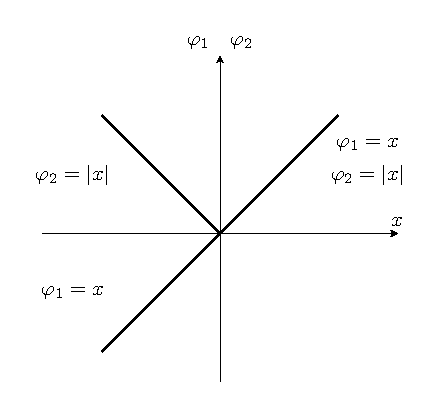
\includegraphics[width=0.5\textwidth]{Imagenes/Ejercicio_Opcional_07.eps}
\end{center}
\caption{Gráfica de las funciones $x$ y $\abs{x}$}
\label{fig:figura_09_03}
\end{wrapfigure}

La función $sgn x$ es el signo de $x$. Ya que $\ptilde{\varphi}_{1} = 1$ y $\ptilde{\varphi}_{2} = sng \, x$, se tiene que: $W(\varphi_{1}, \varphi_{2}) = 0$ para cualquier intervalo, incluyendo $[-1, +1]$.
\\[0.5em]
Que el Wronskiano en el intervalo $[-1, +1]$: ¿prueba eso que $\varphi_{1}$ y $\varphi_{2}$ sean linealmente dependientes?. 
\\[0.5em]
En la figura se nota claramente que no lo son. ¿Qué es lo que está mal en el argumento?
\end{minipage}
\item Identifica el(los) punto(s) singular(es) y en caso de que sea conducente, con el método de Frobenius resuelve las siguientes ecuaciones diferenciales, las cuales deben de contar con las correspondientes dos soluciones linealmente independientes.
\begin{enumerate}[label=\alph*)]
%Ref. Duffy Pag. 480 6)
\item $x^{2} (1 - x^{2}) \sderivada{y} - 5 \, x \, \pderivada{y} + 9 \, y = 0$
\item $x^{2} \sderivada{y} + x (x^{2} - 1) \pderivada{y} + (1 - x^{2}) y = 0$
\end{enumerate}
\item Sea $C$ una curva cerrada y $D$ una región cerrada. Demuestra la siguiente identidad:
\begin{align*}
\scaleint{6ex}_{\bs C} \phi \, \grad{\phi} \cdot \vb{n} \dd{s} = \scaleint{6ex}_{\bs D} \big( \phi \, \laplacian{\phi} + \grad{\phi} \cdot \grad{\phi} \big) \dd{A}
\end{align*}
\end{enumerate}

\end{document}